\section{Siamese Multi-Object Tracking and Embedding}
\label{sec:SiamMOTandFeatureEmb}

% ##############################################################################
\subsection{Motivation}

One of our experiments involved an end-to-end training of the \gls{siammot} model together with a custom head aimed at embeddings based on \gls{roi}-pooled backbone-extracted features for the object \gls{bbox}. The goal was to force the training process into extracting features that are not only satisfactory for detection and tracking but also contain the necessary information to create embeddings for \gls{reid} purposes during the inference.

We strived for simplicity by extending the processing pipeline without altering the existing infrastructure. From the standpoint of implementation, the \gls{siammot} project itself is organized in a proper object-oriented and modular fashion, which made this particular development task easy in this aspect. However, as we will discuss further, we encountered setbacks in terms of training stability and we had to take appropriate measures. Furthermore, extending a huge model that already requires a significant amount of \gls{gpu} \gls{vram} made it even more demanding.

During the research related to our Siamese tracking survey~\cite{ondrasovic2021siamese}, we noticed one work where the exemplar features were projected using \gls{gap} operation into an embedding space consisting of fewer dimensions~\cite{li2020figsiam}. The embedding vector was produced using the feature tensor that represents the kernel for the cross-correlation operation utilized by the majority of the Siamese trackers discussed so far.

More concretely, suppose the extracted features were represented by a tensor of shape $8 \times 8 \times 256$. Then, the \gls{gap} operation along the channel dimension would produce a tensor of shape $1 \times 1 \times 256$, which could then be further flattened into a single $256$-dimensional vector. In the end, the obtained vector was $l_2$-normalized and thus projected onto a unit hypersphere. In the work of Li~\etal{}~\cite{li2020figsiam}, these embedding vectors were exploited for template updating and for combining multiple templates within a pool of size $n$ in an exponential fashion.

This observation led us to the following hypothesis. Given the fact the Siamese exemplar features do contain some, although probably not sufficient information for pure object \gls{reid}, would it be possible to map them further using a non-linear function to produce embedding vectors that could serve for \gls{reid}? Such features are just a learned template, therefore, some notion of similarity needs to be already built into it.

% ##############################################################################
\subsection{Feature Embedding Head Architecture}

% ------------------------------------------------------------------------------
\begin{figure}[!t]
    \centering
    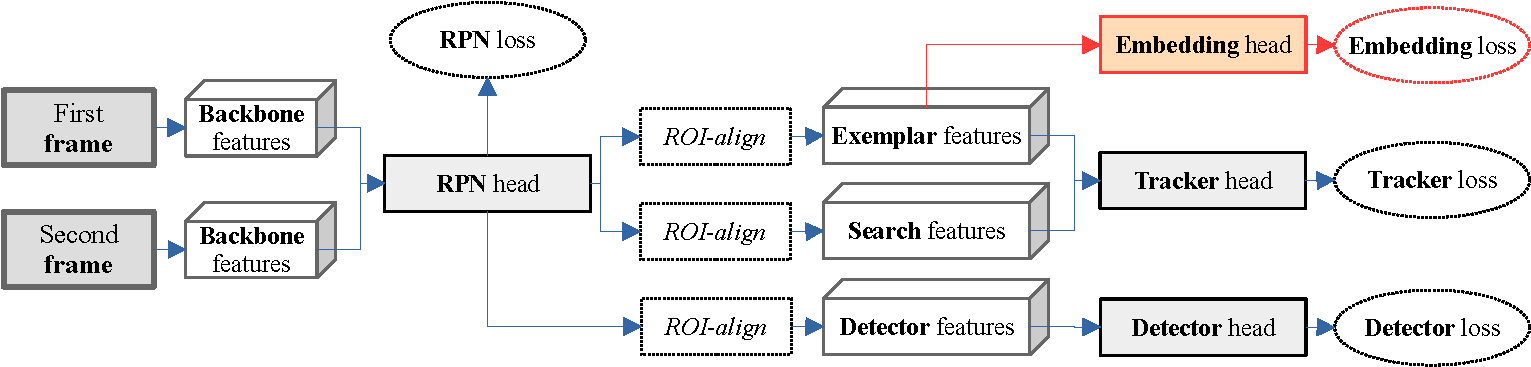
\includegraphics[width=\linewidth]{figures/siamese_tracking/siammot_feature_emb_training.pdf}
    \caption[Embedding-enhanced \gls{siammot} architecture]{Our extension (shown in red) to the underlying \gls{siammot} architecture that incorporates vector embeddings to the end-to-end training. This diagram shows the pipeline that is used during the training, not inference.}
    \label{fig:SiamMOTWithEmbeddings}
\end{figure}
% ------------------------------------------------------------------------------

As far as the vector embedding computation was concerned, we attached the embedding head (\tabletext{}~\ref{tab:FeatureEmbeddingHead}) into the backbone features but after the \gls{roi}-pooling operation (\figtext{}~\ref{fig:SiamMOTWithEmbeddings}). This ensured fixed tensor shapes and allowed us to process the very same features that the object detector and Siamese tracker utilized, too. Simply put, for every proposal made for a particular frame, we looked at the delineated \gls{bbox} through the lens of \gls{roi}-pooling to extract backbone features. In fact, we simply reused the extracted exemplar features. Later on, we processed these features using our newly devised embedding head to produce feature embeddings. The resulting embeddings were subjected to the triplet loss computation (discussed next) with all the necessary operations such as various types of hard negative mining.

\begin{table}[!t]
    \centering
    \begin{tabular}{lll}
        \toprule
        \textbf{layer}    & \textbf{tensor shape}        & \textbf{parameters no.} \\
        \midrule
        input             & $\sbrackets{B, 256, 15, 15}$ & $0$                     \\
        \midrule
        conv $3 \times 3$ & $\sbrackets{B, 256, 13, 13}$ & $589\ 824$              \\
        ReLU              & $\sbrackets{B, 256, 13, 13}$ & $0$                     \\
        \midrule
        conv $3 \times 3$ & $\sbrackets{B, 512, 11, 11}$ & $1\ 179\ 648$           \\
        ReLU              & $\sbrackets{B, 512, 11, 11}$ & $0$                     \\
        \midrule
        flatten           & $\sbrackets{B, 61952}$       & $0$                     \\
        linear            & $\sbrackets{B, 1024}$        & $63\ 439\ 872$          \\
        \midrule
        $l_2$-normalize   & $\sbrackets{B, 1024}$        & $0$                     \\
        \bottomrule
                          & \textbf{total}               & $65\ 209\ 344$          \\
        \cline{2-3}
    \end{tabular}
    \caption[Feature embedding head]{Our custom embedding head that we used to process backbone-extracted features to produce embedding vectors. It is built from two convolutional layers separated by a \gls{relu} nonlinearity followed by a fully connected layer which produces a $1024$ dimensional feature embedding. The batch size dimension is given by $B$ in the tensor shape. Since each embedding vector is normalized to unit length, we avoided learning biases throughout the whole network.}
    \label{tab:FeatureEmbeddingHead}
\end{table}

% ##############################################################################
\subsection{Training Phase}

The training phase was altered by adding another loss function to the sum of already existing three losses from the original model. In particular, the general \gls{siammot} loss function defined in \eqtext{}~\ref{eq:SiamMOTGeneralLoss} was reformulated as
\begin{equation}
    \label{eq:SiamMOTFeatureEmbLoss}
    \lossf = l_{rpn} + l_{detect} + l_{motion} + l_{emb}.
\end{equation}
The $l_{emb}$ loss incorporated triplet loss (\eqtext{}~\ref{eq:TripletLoss} on page~\pageref{eq:TripletLoss}). We also experimented with the contrastive loss (\eqtext{}~\ref{eq:ContrastiveLoss} on page~\pageref{eq:ContrastiveLoss}), but the effect was detrimental in every aspect, so we will not discuss it any further. As we remarked in \sectiontext{}~\ref{sec:LatentSpacesAndEmbeddings} on page \pageref{sec:LatentSpacesAndEmbeddings} aimed at latent spaces and embeddings, it is crucial to adopt appropriate sample mining strategies when using the triplet loss. The rationale is that for the training to keep progressing, the model needs to encounter harder and harder triplets to generate sufficient learning signals. To this end, we went for the semi-hard triplet mining strategy (\eqtext{}~\ref{eq:BatchHardMining} on page~\pageref{eq:BatchHardMining}). However, we struggled with collapsing embeddings~\cite{levi2021rethinking}. This phenomenon happens when the embedding training forces the model to project all the features onto a single point in the embedding space, thus incurring the loss equal to the used margin. We claim that the use of semi-hard negative mining produced triplets that were too difficult. Since we used all the \gls{rpn} proposals to generate triplets, one may imagine that there would always be proposals covering only some small part of the object, making it problematic for the network to learn the concept of ``similarity'' and ``difference'' if it only processes very hard images. Nevertheless, these situations are very common in margin-based losses~\cite{levi2021rethinking}. The computed loss is so high that it is more suitable for the model to map all the features onto a single embedding vector. To remedy this, we implemented batch-all online mining strategy (\eqtext{}~\ref{eq:BatchAllLossFunction} on page \pageref{eq:BatchAllLossFunction}), which stabilized the training. We recommend first utilizing batch-all mining strategy during the training, and then slowly proceeding to batch-hard strategy after a certain point. We still have not implemented this approach, because it would be time-consuming to find the right hyperparameters. There are many open questions, such as to mine the \gls{rpn} proposals in a better way or to set the margin to a higher value. Loss functions aimed at object \gls{reid} are notoriously cumbersome to train. One last remark is that we implemented the entire mining algorithm followed by the loss computation in a \gls{gpu}-only fashion for fast execution and easy integration into the pipeline.

% ##############################################################################
\subsection{Inference Phase}

\subsubsection{Feature-based Non-Maximum Suppression}
\label{sssec:FeatureNonMaximumSuppression}

Salscheider~\cite{salscheider2020featurenms} proposed an extended \gls{nms} algorithm that incorporates a distance between feature embeddings dubbed as \featurenms{}. Considering our idea introduced above, we had to encompass the vector embeddings into the solver reasoning. In the beginning, we came up with the solution that exactly copied the one the mentioned author proposed. That provided further justification for attempting to implement the algorithm and test it in practice. The advantage is that this approach is restricted to the inference phase, thus experimenting with it did not require model re-training.

We assume the reader is acquainted with the original \gls{nms} algorithm (more in \sectiontext{}~\ref{ssec:NonMaximumSuppression}.). Nevertheless, here we repeat the same definitions for clarity. Let $\mset{B} = \cbrackets{\vect{b}_1, \vect{b}_2, \dots, \vect{b}_n}$ be a set of $n$ region proposals described by $n$ \glspl{bbox}. Scores for each detection are contained in a set $\mset{S} = \cbrackets{s_1, s_2, \dots, s_n}$, where $s_i$ denotes a detection score for the $i$-th box, $\vect{b_i}$. This time, we are also going to need the associated feature embedding vectors with each \gls{bbox}, represented by a set $\mset{E} = \cbrackets{\vect{e}_1, \vect{e}_2, \dots, \vect{e}_n}$. Let $\mset{B}_{fnms}$ be  the set of filtered proposal instances from the set $\mset{B}$ produced using the \featurenms{} algorithm.

\def\threshlower{\tau_{\text{lower}}}
\def\threshupper{\tau_{\text{upper}}}
\def\threshsim{\delta}

The distinction in terms of parameters is the following. The original algorithm required only one threshold for the maximum allowed portion of the overlap between regions. The \featurenms{} requires three parameters discussed below.
\begin{itemize}
    \item A minimum threshold $\threshlower$ denoting the boundary below which the two objects are deemed as different. This value should be low, for example, $0.2$, which means that if the \gls{iou} between the two objects is less than $0.2$, then the two instances should be treated as different objects.
    \item A maximum threshold $\threshupper$ denoting a boundary above which the two objects are considered to be identical. Conversely to the $\threshlower$, this value should be high, for instance, $0.8$, which indicates that if the \gls{iou} of the two object instances surpasses this threshold, then it should be the same object, and thus, the \gls{bbox} with the lower confidence is discarded.
    \item A threshold $\threshsim$ is used as a decision boundary between the embedding vectors. This threshold should reflect a measure of similarity. If the adopted measure of similarity (cosine distance, Euclidean distance, ...) falls below $\threshsim$, then the two objects are different, otherwise, they are considered the same one. This value of $\threshsim$ is used only if the two conditions above do not hold.
\end{itemize}

Here we provide a pseudocode of the \featurenms{} algorithm:

\begin{algorithmic}[1]
    \Function{Feature-NMS}{$\mset{B}$, $\mset{S}$, $\mset{E}$, $\threshlower$, $\threshupper$, $\threshsim$}

    \State $\mset{B}_{fnms}$ $\gets$ $\emptyset$
    \Comment{initialize the output (filtered) set of region proposals}

    \While {$\mset{B} \neq \emptyset$}
    \Comment{loop until all the proposals are processed}

    \State $m \gets \underset{i \in \cbrackets{1, 2, \dots, \msetsize{S}}}{\argmax{}} \mset{S}$
    \Comment{find an index of a proposal with the highest score}

    \State $\mset{B} \gets \mset{B} - \vect{b}_m$, $\mset{S} \gets \mset{S} - s_m$, $\mset{E} \gets \mset{E} - \vect{e}_m$
    \Comment{remove the proposal}

    \State $\mset{B}_{fnms} \gets \mset{B}_{fnms} \cup \vect{b}_m$
    \Comment{save the proposal with the highest score}

    \For{$i \gets 1$ to $\msetsize{B}$}
    \Comment{iterate through remaining proposals}

    \If{\Call{iou}{$\vect{b}_m$, $\vect{b}_i$} $\geq \threshlower$}
    \Comment{above the lower-bound threshold}

    \If{\Call{iou}{$\vect{b}_m$, $\vect{b}_i$} $\geq \threshupper$}
    \Comment{above the upper-bound threshold}

    \State $\mset{B} \gets \mset{B} - \vect{b}_i$, $\mset{S} \gets \mset{S} - s_i$, $\mset{E} \gets \mset{E} - \vect{e}_i$
    \Comment{remove the proposal}

    \Else

    \If{\Call{similarity}{$\vect{e}_m$, $\vect{e}_i$} $\geq \threshsim$}
    \Comment{similarity above threshold}
    \State $\mset{B} \gets \mset{B} - \vect{b}_i$, $\mset{S} \gets \mset{S} - s_i$, $\mset{E} \gets \mset{E} - \vect{e}_i$
    \Comment{remove the proposal}
    \EndIf

    \EndIf
    \EndIf
    \EndFor
    \EndWhile

    \State \Return $\mset{B}_{fnms}$
    \EndFunction
\end{algorithmic}

% ##############################################################################
\subsection{Experimental Evaluation and Discussion}

The proposed embedding-based enhancement was evaluated against the baseline model without the embedding head. For a fair comparison, we made sure that all the hyperparameters were identical. The only hyperparameter that we had to change compared to the original model was the batch size. Since the triplet loss requires computation of a great number of triplets, especially the batch-all strategy, we had to decrease the batchsize to avoid crashes due to not having enough \gls{gpu} \gls{vram} available.

We ackowledge that it is diffcult to compare the baseline model with the proposed extension since they progress differently during the training. Therefore, we saved the model state after $K$ training iterations and then evaluated the performance using the validation dataset. We repeated the same process for the baseline architecture, which we trained it from scratch using smaller batch sizes. Furthermore, the embedding evaluation also requires the cosine similarity threshold. We tried multiple different values to see the effect.

\todo[inline]{Add $2$D scatter plot with the baseline vs. embedding - \gls{mota} vs. \gls{motp}.}
\todo[inline]{Add $2$D scatter plot with the baseline vs. embedding - precision vs. recall.}

% ##############################################################################
\subsection{Discussion}

We conjecture that our inability to improve the tracker performance was not particularly caused by the feature embedding itself. There is a recently published work Lu~\etal{}~\cite{lu2020retinatrack}, who introduced their \retinatrack{} tracker. This framework exploited the base visual object detector called a \retinanet{}~\cite{lin2018focal} and then added, in principle, the same head as we did for the purpose of producing feature embeddings that could be used for \gls{reid}. However, there are obvious differences between the two trackers in terms of how the inference phase is executed, and that is where we see the root cause of our failure.
